%%%%%%%%%%%%%%%%%%%%%%%%%%%%%%%%%%%%%%%%%%%%%%%%%%%%%%%%%%%%%%%%%%%%%%%%%%%%%%%%
%
% Template license:
% CC BY-NC-SA 3.0 (http://creativecommons.org/licenses/by-nc-sa/3.0/)
%
%%%%%%%%%%%%%%%%%%%%%%%%%%%%%%%%%%%%%%%%%%%%%%%%%%%%%%%%%%%%%%%%%%%%%%%%%%%%%%%%

%----------------------------------------------------------------------------------------
%	PACKAGES AND OTHER DOCUMENT CONFIGURATIONS
%----------------------------------------------------------------------------------------

\documentclass[
11pt, % The default document font size, options: 10pt, 11pt, 12pt
%oneside, % Two side (alternating margins) for binding by default, uncomment to switch to one side
%chapterinoneline,% Have the chapter title next to the number in one single line
spanish,
singlespacing, % Single line spacing, alternatives: onehalfspacing or doublespacing
%draft, % Uncomment to enable draft mode (no pictures, no links, overfull hboxes indicated)
%nolistspacing, % If the document is onehalfspacing or doublespacing, uncomment this to set spacing in lists to single
%liststotoc, % Uncomment to add the list of figures/tables/etc to the table of contents
%toctotoc, % Uncomment to add the main table of contents to the table of contents
parskip, % Uncomment to add space between paragraphs
%codirector, % Uncomment to add a codirector to the title page
headsepline, % Uncomment to get a line under the header
]{MastersDoctoralThesis} % The class file specifying the document structure



%----------------------------------------------------------------------------------------
%	INFORMACIÓN DE LA MEMORIA
%----------------------------------------------------------------------------------------

\thesistitle{Desarrollo de un chatbot especializado para optimizar la búsqueda de información en documentos propietarios} % El títulos de la memoria, se usa en la carátula y se puede usar el cualquier lugar del documento con el comando \ttitle

% Nombre del posgrado, se usa en la carátula y se puede usar el cualquier lugar del documento con el comando \degreename
\posgrado{Carrera de Especialización en Inteligencia Artificial} 

\author{Ing. Fabián Alejandro Massotto} % Tu nombre, se usa en la carátula y se puede usar el cualquier lugar del documento con el comando \authorname

\director{Esp. Ing. Ezequiel Guinsburg (FIUBA)} % El nombre del director, se usa en la carátula y se puede usar el cualquier lugar del documento con el comando \dirname
%\codirector{} % El nombre del codirector si lo hubiera, se usa en la carátula y se puede usar el cualquier lugar del documento con el comando \codirname.  Para activar este campo se debe descomentar la opción "codirector" en el comando \documentclass, línea 23.

\juradoUNO{Nombre del jurado 1 (pertenencia)} % Nombre y pertenencia del un jurado se usa en la carátula y se puede usar el cualquier lugar del documento con el comando \jur1name
\juradoDOS{Nombre del jurado 2 (pertenencia)} % Nombre y pertenencia del un jurado se usa en la carátula y se puede usar el cualquier lugar del documento con el comando \jur2name
\juradoTRES{Nombre del jurado 3 (pertenencia)} % Nombre y pertenencia del un jurado se usa en la carátula y se puede usar el cualquier lugar del documento con el comando \jur3name

\ciudad{Ciudad Autónoma de Buenos Aires}

\fechaINICIO{abril de 2024}
\fechaFINAL{abril de 2025}


\keywords{inteligencia artificial, chatbot,  FIUBA} % Keywords for your thesis, print it elsewhere with \keywordnames


\begin{document}


\frontmatter % Use roman page numbering style (i, ii, iii, iv...) for the pre-content pages

\pagestyle{plain} % Default to the plain heading style until the thesis style is called for the body content


%----------------------------------------------------------------------------------------
%	RESUMEN - ABSTRACT 
%----------------------------------------------------------------------------------------

\begin{abstract}
\addchaptertocentry{\abstractname} % Add the abstract to the table of contents
%
%The Thesis Abstract is written here (and usually kept to just this page). The page is kept centered vertically so can expand into the blank space above the title too\ldots
\centering

El presente trabajo aborda el desarrollo de un chatbot que interpreta consultas realizadas en lenguaje natural y ofrece respuestas precisas basadas en documentos empresariales previamente procesados. Su valor radica en la eficiencia operativa que se obtiene al optimizar el acceso a información crítica de una organización.				

En esta memoria se detallan todas las etapas del desarrollo, desde la preparación de los datos hasta la evaluación del rendimiento del chatbot. Para lograrlo, se aplicaron conocimientos de procesamiento de lenguaje natural, modelos grandes de lenguaje e inteligencia artificial generativa.				
\end{abstract}

%----------------------------------------------------------------------------------------
%	CONTENIDO DE LA MEMORIA  - AGRADECIMIENTOS
%----------------------------------------------------------------------------------------

%\begin{acknowledgements}
%\addchaptertocentry{\acknowledgementname} % Descomentando esta línea se puede agregar los agradecimientos al índice
%\vspace{1.5cm}
%
%Esta sección es para agradecimientos personales y es totalmente \textbf{OPCIONAL}.  
%
%\end{acknowledgements}

%----------------------------------------------------------------------------------------
%	LISTA DE CONTENIDOS/FIGURAS/TABLAS
%----------------------------------------------------------------------------------------

\tableofcontents % Prints the main table of contents

\listoffigures % Prints the list of figures

\listoftables % Prints the list of tables


%----------------------------------------------------------------------------------------
%	CONTENIDO DE LA MEMORIA  - DEDICATORIA
%----------------------------------------------------------------------------------------

%\dedicatory{\textbf{Dedicado a... [OPCIONAL]}}  % escribir acá si se desea una dedicatoria

%----------------------------------------------------------------------------------------
%	CONTENIDO DE LA MEMORIA  - CAPÍTULOS
%----------------------------------------------------------------------------------------

\mainmatter % Begin numeric (1,2,3...) page numbering

\pagestyle{thesis} % Return the page headers back to the "thesis" style

% Incluir los capítulos como archivos separados desde la carpeta Chapters

% Chapter 1

\chapter{Introducción general} % Main chapter title

\label{Chapter1} % For referencing the chapter elsewhere, use \ref{Chapter1} 
\label{IntroGeneral}

%----------------------------------------------------------------------------------------

% Define some commands to keep the formatting separated from the content 
\newcommand{\keyword}[1]{\textbf{#1}}
\newcommand{\tabhead}[1]{\textbf{#1}}
\newcommand{\code}[1]{\texttt{#1}}
\newcommand{\file}[1]{\texttt{\bfseries#1}}
\newcommand{\option}[1]{\texttt{\itshape#1}}
\newcommand{\grados}{$^{\circ}$}

%----------------------------------------------------------------------------------------

En este capítulo se introduce la problemática que motivó el presente trabajo, seguida de una breve descripción de la solución propuesta. 
A continuación, se expone el estado del arte de las tecnologías aplicadas. 
Finalmente, se detallan el alcance y los requerimientos necesarios para su implementación.

%----------------------------------------------------------------------------------------
\section{Marco de la propuesta}

En un entorno empresarial, la eficiencia en la búsqueda de información es crucial para la
productividad y el rendimiento de los empleados. Sin embargo, con la creciente cantidad de
datos y documentos disponibles, encontrar información específica de manera rápida y precisa
puede convertirse en un desafío.

La abundancia de fuentes de información, lejos de agilizar el trabajo, a menudo lo complica. En una empresa, 
es común que existan múltiples repositorios de documentos, políticas y datos históricos, pero la falta de centralización y la 
dificultad para identificar la fuente correcta suelen traducirse en pérdidas de tiempo significativas. 
En muchas ocasiones, se dedica más tiempo a la búsqueda de información que a la ejecución de las tareas 
en sí, lo que afecta tanto la productividad como la efectividad en la toma de decisiones.

El presente trabajo surgió como un desarrollo personal para abordar esta problemática. Su propósito fue 
proponer una solución que facilite el acceso ágil y preciso a la información necesaria, de manera tal
que optimice el uso del tiempo en un entorno con gran cantidad de fuentes de información.

Un chatbot especializado ofrece una solución prometedora al permitir a los usuarios realizar 
consultas en lenguaje natural y obtener respuestas de manera instantánea. Mientras que otros sistemas 
de inteligencia artificial ampliamente conocidos y utilizados 
destacan en su capacidad para generar respuestas generales basadas en un amplio conocimiento del 
lenguaje, el presente trabajo se distingue por su capacidad para trabajar con documentos altamente 
específicos (y potencialmente privados). Esto le permite ofrecer respuestas adaptadas al contexto 
interno de la organización, que no podrían obtenerse mediante el uso de los chatbots de 
propósito general disponibles en el mercado \citep{website:chatgpt} \citep{website:copilot} \citep{website:gemini}.

En la figura \ref{fig:diagrama-bloques-basico} se presenta un diagrama de alto nivel de la solución.
En primer lugar, los usuarios interactúan con el chatbot a través de una interfaz gráfica desde donde
pueden realizar consultas sobre la información deseada. Estas consultas, procesadas mediante 
técnicas de lenguaje natural, permiten extraer la información más relevante de la fuente de documentos. 
Luego, un modelo de inteligencia artificial interpreta las consultas y genera respuestas que proporcionan 
al usuario la información solicitada de manera precisa y contextualizada.

\begin{figure}[ht]
	\centering
	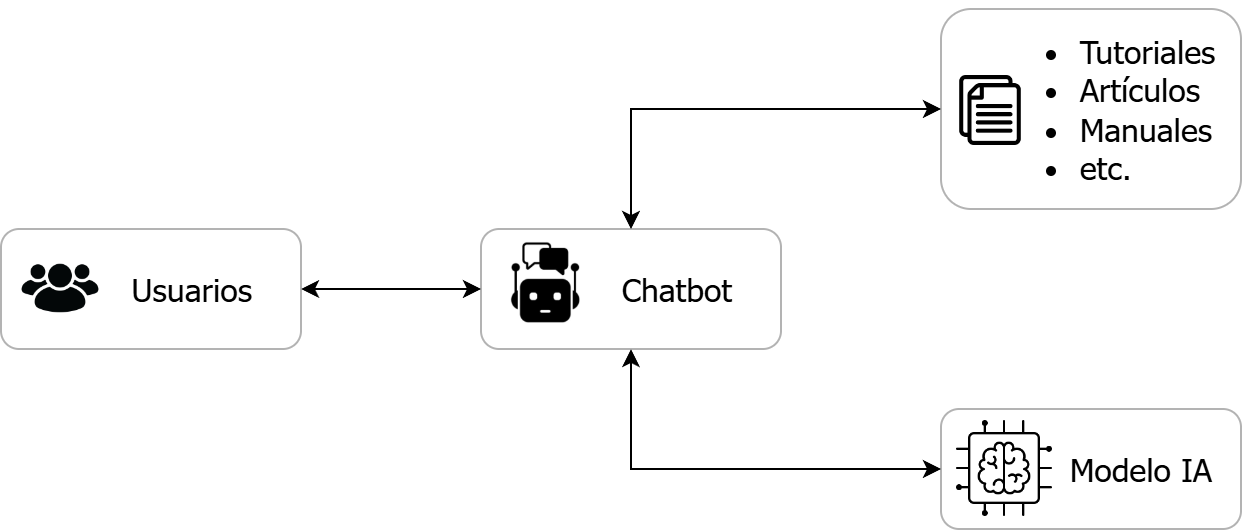
\includegraphics[scale=.3]{./Figures/diagrama_bloques_basico.png}
	\caption{Diagrama de alto nivel de la solución.}
	\label{fig:diagrama-bloques-basico}
\end{figure}

\vspace{15mm}

%----------------------------------------------------------------------------------------
\section{Estado del arte}

El desarrollo de chatbots y sistemas de recuperación de información ha avanzado considerablemente en los últimos años, 
impulsado por mejoras en el procesamiento de lenguaje natural (NLP, por su sigla en inglés) y el acceso a grandes volúmenes de datos. 
En este contexto, los chatbots especializados han surgido como soluciones destacadas para el acceso eficiente 
a información específica en distintos entornos, incluyendo el empresarial. A continuación, se presenta una revisión 
de las principales tecnologías y enfoques actuales que sustentan el desarrollo del presente trabajo.

Los chatbots modernos han evolucionado desde sistemas de reglas simples hasta modelos sofisticados capaces de 
mantener conversaciones complejas. Entre los primeros desarrollos, como ELIZA \citep{paper:eliza} en 
la década de 1960, se empleaban reglas predefinidas que limitaban la interacción a una cantidad pequeña de 
respuestas posibles. Sin embargo, el uso de redes neuronales y el aprendizaje profundo en las últimas décadas 
han revolucionado el campo, al permitir la aparición de sistemas como Siri de Apple, Alexa de Amazon 
y Google Assistant \citep{article:voice-assistants}. Estos asistentes virtuales han popularizado el uso de interfaces 
de conversación en la vida cotidiana, ya que son capaces de responder a preguntas comunes, realizar tareas administrativas 
y ofrecer asistencia en tiempo real.

Una tendencia reciente en el desarrollo de chatbots es la aplicación de modelos generativos de lenguaje, como GPT-3 y GPT-4 
de OpenAI \citep{paper:gpt}, BERT de Google \citep{paper:bert}, y LLAMA de Meta \citep{paper:llama}. Estos modelos, basados 
en arquitecturas de \textit{transformers} \citep{paper:transformers}, permiten una comprensión profunda del contexto y del 
significado en secuencias de palabras. Su capacidad de generar respuestas coherentes y bien estructuradas ha llevado al 
desarrollo de los tan populares chatbots modernos como ChatGPT \citep{website:chatgpt}, Microsoft Copilot \citep{website:copilot}
o Google Gemini \citep{website:gemini}, cuyas interfaces se observan en la figura \ref{fig:chatbots}.

\vspace{25mm}

\begin{figure}[ht]
	\centering
	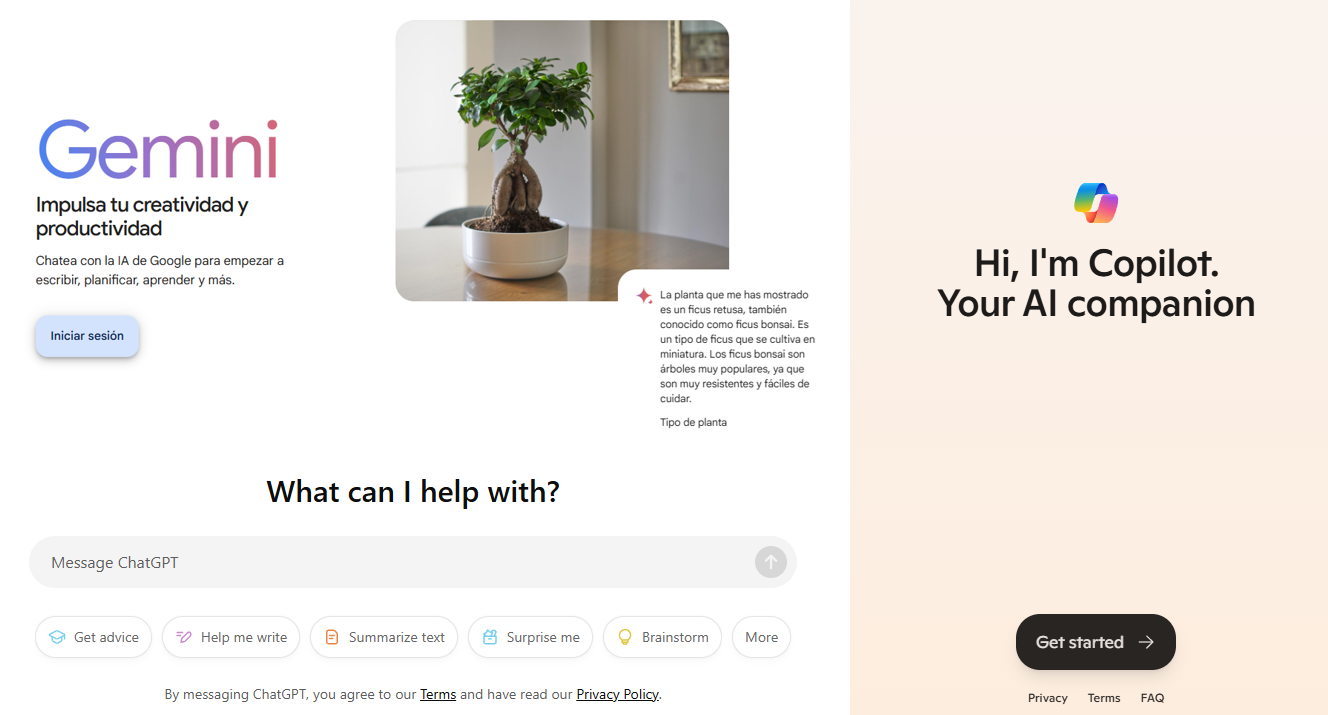
\includegraphics[scale=.38]{./Figures/chatbots.png}
	\caption{ChatGPT, Gemini y Copilot, los chatbots más populares actualmente.}
	\label{fig:chatbots}
\end{figure}

\vspace{10mm}

Si bien los modelos generativos han alcanzado un alto grado de sofisticación, presentan algunas limitaciones importantes. 
En primer lugar, su conocimiento es en gran medida de propósito general, dado que han sido entrenados con grandes volúmenes 
de datos públicos y no específicos, lo que limita su precisión cuando se requiere información particular de una organización. 
En segundo lugar, estos modelos tienden a ``inventar'' respuestas cuando no encuentran información relevante, fenómeno conocido 
como \textit{hallucinations} \citep{article:hallucinations}. En un contexto empresarial, esto puede provocar confusión o incluso 
proporcionar información errónea.

En la búsqueda de soluciones que combinen la capacidad de los modelos generativos con la precisión de la información propietaria, 
ha surgido el enfoque de generación aumentada por recuperación (RAG, por su sigla en inglés). Este enfoque combina sistemas de 
recuperación de información con modelos de generación de texto, lo que permite que las respuestas no solo se basen en la capacidad 
generativa del modelo, sino también en una búsqueda previa en bases de datos o documentos específicos \citep{paper:rag-1} 
\citep{paper:rag-2}.

El presente trabajo se apoya en el estado del arte de los modelos de lenguaje y la técnica de RAG para crear una solución innovadora.

\vspace{10mm}

%----------------------------------------------------------------------------------------
\section{Objetivos y alcance}

El propósito de este trabajo fue optimizar el proceso de búsqueda de información por parte de los empleados. Se buscó
proporcionar una herramienta eficaz que permita acceder rápidamente a los datos relevantes, que mejore la eficiencia y 
productividad en el entorno laboral.

Para ello, se realizaron las siguientes tareas:

\begin{itemize}
	\item Procesamiento de los documentos y posterior almacenamiento en una base de datos.
	\item Integración con un modelo lingüístico grande (LLM) que pueda entender las consultas de los usuarios y proporcionar respuestas precisas basadas en el contenido de los documentos ingestados.
	\item Diseño e implementación de una interfaz de usuario intuitiva y fácil de utilizar que permita a los empleados interactuar con el chatbot de manera eficiente.
	\item Desarrollo de un \textit{pipeline} de despliegue continuo que facilite la ingesta de nuevos documentos y la actualización de la aplicación.
  \item Evaluación del rendimiento del chatbot mediante pruebas exhaustivas con diferentes tipos de consultas.
\end{itemize}

\vspace{5mm}

Las siguientes actividades no formaron parte del alcance:

\begin{itemize}
	\item Despliegue del chatbot en un ambiente productivo.
	\item Entrenamiento continuo del chatbot en base a las consultas realizadas por los usuarios.
	\item Desarrollo de funcionalidades avanzadas de seguridad, tales como autenticación de usuarios o cifrado de datos.
\end{itemize}

\vspace{10mm}

%----------------------------------------------------------------------------------------
\section{Requerimientos}

A continuación se describen los principales requerimientos establecidos durante la etapa de planificación:

\begin{enumerate}
	\item Requerimientos funcionales:
		\begin{enumerate}
			\item El sistema debe permitir a los usuarios consultar por información a través de una interfaz gráfica.
			\item El sistema debe ser capaz de entender consultas escritas en lenguaje natural.
			\item El sistema debe proporcionar respuestas precisas basadas en el contenido de los documentos procesados.
		\end{enumerate}
	\item Requerimientos de la interfaz:
		\begin{enumerate}
	  		\item La interfaz gráfica debe ser intuitiva y fácil de usar para los usuarios.
	  		\item Se debe proporcionar retroalimentación instantánea al usuario luego de realizar una consulta.
	  	\end{enumerate}
	\item Requerimiento de testing:
	  	\begin{enumerate}
	  		\item Se deben realizar pruebas exhaustivas para garantizar la precisión y la robustez del sistema.
	  	\end{enumerate}
	\vspace{10mm}
	\item Requerimientos de documentación:
		\begin{enumerate}
			\item Se deben documentar las pruebas realizadas y los resultados obtenidos.
			\item Se debe elaborar un informe de avance del proyecto.
			\item Se debe confeccionar una memoria técnica del proyecto.
		\end{enumerate}
	\item Requerimientos de cumplimiento normativo:
		\begin{enumerate}
			\item El sistema debe cumplir con las regulaciones de privacidad de datos vigentes.
		\end{enumerate}
\end{enumerate}
\chapter{Introducción específica} % Main chapter title

\label{Chapter2}

%----------------------------------------------------------------------------------------

Este capítulo presenta las técnicas y herramientas clave utilizadas en el 
desarrollo de este trabajo. Se analizan los enfoques fundamentales para el procesamiento de 
lenguaje natural, junto con los modelos, frameworks e infraestructura necesarios para 
construir un sistema de recuperación de información eficiente y escalable. Este recorrido 
técnico permite comprender los fundamentos sobre los que se apoya la solución implementada. 

%---------------------------------------------------------------------------------------
\section{Técnicas de procesamiento de lenguaje natural}

El procesamiento de lenguaje natural (NLP) es un área de la inteligencia artificial que les permite 
a las máquinas comprender e interpretar el lenguaje humano \citep{book:nlp}. Esto juega un papel esencial 
para que un chatbot interprete las consultas de los usuarios y localice la información relevante en los 
documentos procesados. Las técnicas de NLP aplicadas contribuyen a que el sistema entienda el 
significado de las solicitudes, independientemente de variaciones lingüísticas o de sintaxis. Entre los 
métodos de mayor importancia para este trabajo se encuentran los \textit{word embeddings} y los
\textit{transformers}.

\subsection{\textit{Word embeddings}}

Los \textit{embeddings} son una poderosa técnica para transformar datos complejos en formas numéricas que 
son fácilmente procesadas y analizadas por algoritmos de aprendizaje automático \citep{paper:embeddings}. Esta técnica permite 
representar virtualmente cualquier tipo de dato como vectores, lo que posibilita su manipulación en tareas de 
procesamiento de lenguaje natural.

Sin embargo, no se trata solo de convertir las palabras en vectores. Es crucial preservar el significado original 
de los datos para que las tareas realizadas en este espacio transformado mantengan la coherencia semántica. 
Por ejemplo, al comparar dos frases, no solo se desea analizar las palabras que contienen, sino también evaluar 
si ambas expresan un significado similar.

Para conservar el significado, es necesario generar vectores donde las relaciones entre ellos sean representativas 
del contenido. Para ello, se emplea un modelo de \textit{embeddings} pre-entrenado, que produce una representación compacta 
de los datos mientras mantiene sus características semánticas. El objetivo es capturar el significado o las relaciones 
semánticas entre los puntos de datos, de modo que los elementos similares se encuentren cercanos en el espacio vectorial y los disímiles estén alejados. 
Por ejemplo, si se consideran las palabras ``rey'' y ``reina'', un \textit{embedding} podría mapear estas palabras en vectores de modo 
que la diferencia entre ``rey' y ``reina'' sea similar a la diferencia entre ``hombre'' y ``mujer'', y reflejar así las 
relaciones semánticas subyacentes.

En este trabajo, se ensayaron diferentes modelos de \textit{embeddings} de OpenAI, Google y Hugging Face, 
cuya evaluación y selección se detallan en el capítulo \ref{Chapter4}.

\subsection{Transformers}

La arquitectura de \textit{transformers} ha revolucionado el procesamiento de lenguaje natural al introducir un mecanismo de \textit{self-attention}, 
que permite a un modelo evaluar la relevancia de cada palabra en una secuencia en relación con las demás \citep{paper:transformers}. Este enfoque 
supera las limitaciones de modelos secuenciales tradicionales, ya que es capaz de procesar palabras en paralelo y captar dependencias de largo alcance 
en el texto. En lugar de analizar cada palabra en un orden específico, el mecanismo de \textit{self-attention} permite que el modelo ``preste atención'' 
a las palabras más relevantes en el contexto de la frase, al asignar pesos a cada una según su importancia relativa en la oración. Gracias a esta capacidad, 
los \textit{transformers} pueden capturar relaciones contextuales complejas y matices semánticos entre las palabras, 
lo que resulta fundamental para tareas como la generación de texto. Esta arquitectura ha hecho posible que los modelos comprendan y generen 
lenguaje natural de una forma mucho más cercana a la comprensión humana. Esta técnica 
ha sido fundamental en el desarrollo de los modelos grandes de lenguaje, que se introducen a continuación.

%----------------------------------------------------------------------------------------
\section{Modelos grandes de lenguaje}

Los modelos grandes de lenguaje (LLM, por su sigla en inglés) son redes neuronales de gran escala, entrenadas 
para comprender y generar texto en lenguaje natural. Estos modelos, basados en arquitecturas de \textit{transformers}, 
están compuestos por millones o incluso billones de parámetros, lo que les permite capturar patrones complejos y 
relaciones contextuales en vastos conjuntos de datos de texto. Los LLM son capaces de realizar múltiples 
tareas de procesamiento de lenguaje natural, como la generación de texto, la traducción 
automática y el resumen de documentos. En la tabla \ref{tab:llms} se presentan 
algunos de los modelos más relevantes en la actualidad \citep{website:lifearchitect}.

\vspace{5mm}

\begin{table}[h]
	\centering
	\caption[Modelos LLM disponibles en el mercado]{Modelos LLM disponibles en el mercado.}
	\begin{tabular}{l c c c}    
		\toprule
		\textbf{Modelo} 	 & \textbf{Creador} 	& \textbf{Año de publicación}  & \textbf{Cant. de parámetros (aprox.)}\\
		\midrule
		GPT-4o               & OpenAI 				& 2024                         & 200 mil millones\\		
		Gemini 1.5      	 & Google				& 2024                         & 1,5 billones\\
		LLaMa 3         	 & Meta				    & 2024                         & 70 mil millones\\
        GPT-4         	     & OpenAI				& 2023                         & 1,76 billones\\
        LLaMa 2         	 & Meta				    & 2023                         & 70 mil millones\\
        Mistral-7B         	 & Mistral AI		    & 2023                         & 7 mil millones\\
        BLOOM         	     & BigScience		    & 2022                         & 176 mil millones\\
        GPT-3.5         	 & OpenAI				& 2022                         & 20 mil millones\\
		\bottomrule
		\hline
	\end{tabular}
	\label{tab:llms}
\end{table}

\vspace{5mm}

En este trabajo, el modelo LLM desempeña un papel central ya que es el encargado de entender las consultas de 
los usuarios y generar respuestas coherentes. Para seleccionar el modelo más adecuado, 
se ensayaron diferentes variantes, cuyos detalles se describen en el capítulo \ref{Chapter4}.

\subsection{Modelos LLM versus modelos tradicionales}

A continuación se mencionan las principales diferencias entre los modelos grandes de lenguaje y los
modelos tradicionales:

\begin{itemize}
	\item Los LLM pueden adaptarse a nuevas tareas simplemente con el empleo de ejemplos en el \textit{prompt}, 
	sin necesidad de modificar sus parámetros o re-entrenar. Esto contrasta con los modelos tradicionales, 
	que requieren grandes conjuntos de datos etiquetados y re-entrenarse cada vez que se incorporan nuevas tareas.
	\item Comprenden instrucciones en lenguaje natural, lo que les permite seguir indicaciones complejas e 
	incluso inferir reglas implícitas a partir de ejemplos. Los modelos tradicionales, en cambio, suelen necesitar 
	formatos de entrada específicos y siguen reglas programadas explícitamente, sin capacidad para inferir patrones 
	nuevos en tiempo real.
	\item Mantienen la coherencia en conversaciones largas y son capaces de recordar información dada en 
	partes previas del diálogo. Los modelos tradicionales procesan cada entrada de manera independiente y no pueden 
	conservar el estado conversacional.
	\item Permiten una interacción bidireccional, donde pueden solicitar aclaraciones y ajustar sus respuestas 
	en función del \textit{feedback} recibido. Los modelos tradicionales, en cambio, ofrecen una interacción unidireccional
	y no manejan \textit{feedback} en tiempo real.
	\item Un solo LLM es capaz de realizar múltiples tareas sin configuración adicional y de adaptar su salida según 
	el contexto. Por el contrario, los modelos tradicionales están diseñados para una tarea específica, por lo que 
	se requiere un modelo separado para cada tarea.
\end{itemize}

%----------------------------------------------------------------------------------------
\section{Generación aumentada por recuperación}

Una limitación importante que presentan los LLM es que, debido a su naturaleza generalista, pueden 
carecer de precisión cuando se aplican a dominios específicos, ya que su conocimiento está limitado a la información 
con la que fueron entrenados. Si bien esta información es sumamente vasta, no alcanza a cubrir la infinidad de temas 
posibles, y no contempla contenido no disponible en fuentes públicas.

Para abordar esta limitación, los LLM pueden adaptarse mediante la técnica conocida como recuperación aumentada por 
generación (RAG) \citep{paper:rag-1}, que integra fuentes de datos especializadas que mejoran su precisión 
en contextos concretos, como el entorno empresarial. De esta manera, los LLM pueden aprovechar su capacidad de 
comprensión profunda del lenguaje, pero también acceder a información precisa y actualizada de documentos específicos.

Básicamente, esta técnica consta de dos fases principales: primero, se realiza una búsqueda entre los documentos
provistos y se seleccionan fragmentos que sean relevantes para la consulta del usuario. Luego, un modelo LLM
utiliza esa información para construir una respuesta contextualizada. En la figura \ref{fig:rag} se ilustra
un diagrama básico de su funcionamiento.

\vspace{3mm}

\begin{figure}[ht]
	\centering
	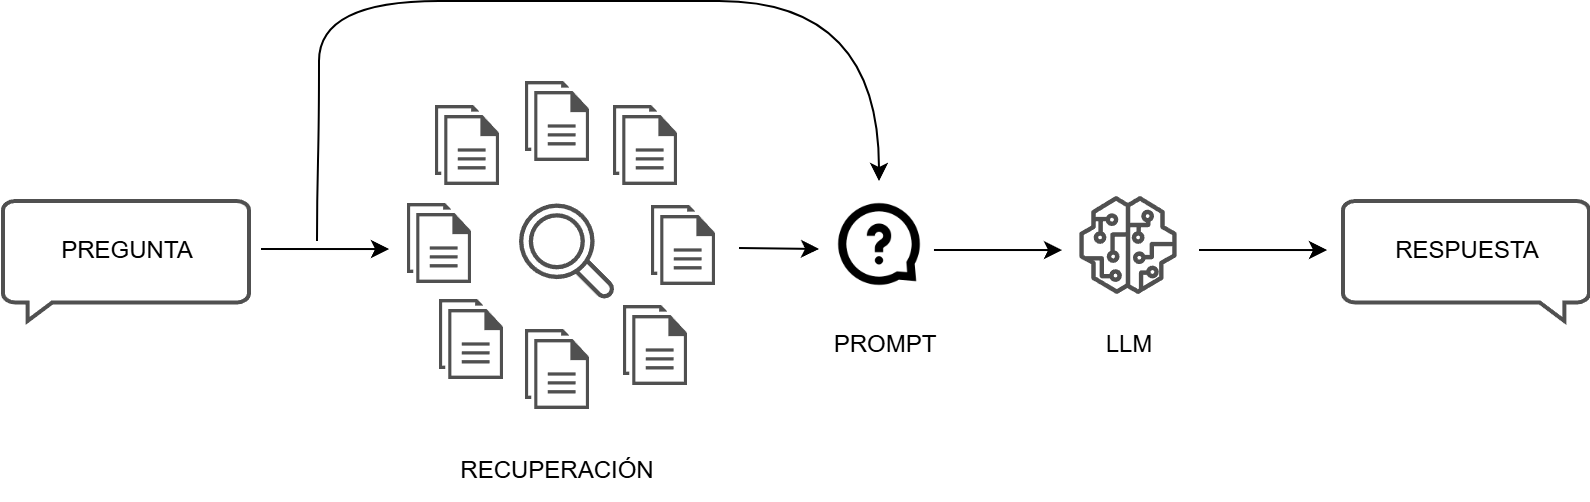
\includegraphics[scale=.24]{./Figures/rag.png}
	\caption{Diagrama de un sistema RAG.}
	\label{fig:rag}
\end{figure}

La combinación de recuperación y generación permite un flujo de información enriquecido, al lograr un equilibrio 
entre las capacidades generales del modelo y la especificidad requerida en el contexto empresarial.

%----------------------------------------------------------------------------------------
\section{Bases de datos vectoriales}

Una base de datos de vectorial \citep{article:vector-db} es un sistema diseñado para almacenar y gestionar \textit{embeddings}. Esta
cumple un papel fundamental en la etapa de recuperación de información.

A diferencia de las bases de datos tradicionales, en las que las consultas suelen coincidir exactamente con los valores almacenados, 
las bases de datos vectoriales aplican métricas de similitud para identificar el vector más cercano a la consulta. 
El proceso de recuperación se realiza mediante el cálculo de la distancia entre 
el vector de la consulta y los vectores almacenados en la base de datos. Los fragmentos con menor distancia al vector 
de la consulta son seleccionados como los más relevantes y luego utilizados como insumo en la fase de generación de la respuesta. 

Para seleccionar la base de datos vectorial más adecuada para este trabajo, se exploraron varias opciones 
disponibles en el mercado y se evaluaron aspectos como el rendimiento y la facilidad de integración con el chatbot. 
Los resultados de estos ensayos se describen en el capítulo \ref{Chapter4}.

%----------------------------------------------------------------------------------------
\section{Frameworks utilizados}

En el desarrollo de este trabajo se utilizaron una serie frameworks que facilitaron la implementación de 
cada parte del sistema. A continuación, se detallan sus principales características y su rol específico en el producto final.

\begin{itemize}
	\item LangChain: este framework es fundamental para la construcción del sistema RAG, ya que permite una gestión 
	eficiente de flujos de trabajo con modelos de lenguaje. LangChain facilita la integración de modelos LLM con fuentes de datos externas, 
	y además ofrece herramientas para diseñar flujos complejos 
	que manejan las consultas del usuario, el proceso de recuperación y la generación de respuestas \citep{website:langchain}.
	\item FastAPI: se utiliza para construir la API que conecta los componentes del sistema y gestiona las solicitudes del usuario. 
	Este framework, reconocido por su alto rendimiento y facilidad de uso, permitió desarrollar una API eficiente y escalable que procesa 
	las consultas en tiempo real. FastAPI facilita el manejo de solicitudes asíncronas y permite definir de manera clara los puntos 
	de conexión de la API, asegurando que las interacciones entre el frontend y el backend se 
	realicen de forma fluida y rápida \citep{website:fastapi}.
	\item NextUI: es un framework de diseño de interfaces de usuario 
	basado en React que permite construir interfaces modernas y responsivas. NextUI facilitó la creación de una interfaz intuitiva 
	y fácil de usar, que permite a los usuarios interactuar con el chatbot de manera fluida. Este framework ofrece una variedad de 
	componentes pre-construidos y altamente personalizables, lo que ayudó a reducir el tiempo de desarrollo de la interfaz y asegurar 
	una experiencia de usuario satisfactoria \citep{website:nextui}.
\end{itemize}

%----------------------------------------------------------------------------------------
\section{Servicios en la nube utilizados}

En este trabajo se empleó Microsoft Azure \citep{website:azure} como la plataforma principal de infraestructura en la nube, seleccionada por su robustez y 
variedad de servicios orientados a aplicaciones de inteligencia artificial. Azure ofrece soluciones 
escalables y seguras para gestionar datos y modelos, lo que facilita la integración de distintos recursos en un entorno controlado y eficiente.

Los recursos específicos de Azure utilizados incluyen:

\begin{itemize}
	\item Azure OpenAI: este recurso se utilizó para deployar el modelo de lenguaje LLM y el modelo de \textit{embeddings}, 
	lo que provee la capacidad de procesamiento de lenguaje natural avanzada requerida por el sistema \citep{website:azure-openai}.
	\item Azure AI Search: utilizado como base de datos vectorial, este servicio permite almacenar y recuperar \textit{embeddings} 
	mediante búsquedas de similitud \citep{website:ai-search}.
	\item Azure App Service: empleado para hospedar el backend del chatbot, este servicio garantiza un entorno seguro y 
	escalable para la ejecución de la API y la gestión de consultas de los usuarios \citep{website:app-service}.
	\item Azure Static Web Apps: utilizado para hospedar el frontend del chatbot, proporciona un despliegue 
	rápido y eficiente de la interfaz de usuario y puede ser accedido por los empleados desde cualquier ubicación \citep{website:static-web-app}.
\end{itemize}

Además, se implementó GitHub Actions \citep{website:github-actions} como \textit{pipeline} de integración y despliegue continuo, no solo para publicar 
actualizaciones del backend y el frontend, sino también para automatizar la actualización del contenido de la base de datos. 
\chapter{Diseño e implementación} % Main chapter title

\label{Chapter3} % Change X to a consecutive number; for referencing this chapter elsewhere, use \ref{ChapterX}

\definecolor{mygreen}{rgb}{0,0.6,0}
\definecolor{mygray}{rgb}{0.5,0.5,0.5}
\definecolor{mymauve}{rgb}{0.58,0,0.82}

%%%%%%%%%%%%%%%%%%%%%%%%%%%%%%%%%%%%%%%%%%%%%%%%%%%%%%%%%%%%%%%%%%%%%%%%%%%%%
% parámetros para configurar el formato del código en los entornos lstlisting
%%%%%%%%%%%%%%%%%%%%%%%%%%%%%%%%%%%%%%%%%%%%%%%%%%%%%%%%%%%%%%%%%%%%%%%%%%%%%
\lstset{ %
  backgroundcolor=\color{white},   % choose the background color; you must add \usepackage{color} or \usepackage{xcolor}
  basicstyle=\footnotesize,        % the size of the fonts that are used for the code
  breakatwhitespace=false,         % sets if automatic breaks should only happen at whitespace
  breaklines=true,                 % sets automatic line breaking
  captionpos=b,                    % sets the caption-position to bottom
  commentstyle=\color{mygreen},    % comment style
  deletekeywords={...},            % if you want to delete keywords from the given language
  %escapeinside={\%*}{*)},         % if you want to add LaTeX within your code
  %extendedchars=true,             % lets you use non-ASCII characters; for 8-bits encodings only, does not work with UTF-8
  %frame=single,	                 % adds a frame around the code
  keepspaces=true,                 % keeps spaces in text, useful for keeping indentation of code (possibly needs columns=flexible)
  keywordstyle=\color{blue},       % keyword style
  language=python,                % the language of the code
  %otherkeywords={*,...},          % if you want to add more keywords to the set
  numbers=left,                    % where to put the line-numbers; possible values are (none, left, right)
  numbersep=5pt,                   % how far the line-numbers are from the code
  numberstyle=\tiny\color{mygray}, % the style that is used for the line-numbers
  rulecolor=\color{black},         % if not set, the frame-color may be changed on line-breaks within not-black text (e.g. comments (green here))
  showspaces=false,                % show spaces everywhere adding particular underscores; it overrides 'showstringspaces'
  showstringspaces=false,          % underline spaces within strings only
  showtabs=false,                  % show tabs within strings adding particular underscores
  stepnumber=1,                    % the step between two line-numbers. If it's 1, each line will be numbered
  stringstyle=\color{mymauve},     % string literal style
  tabsize=2,	                     % sets default tabsize to 2 spaces
  title=\lstname,                  % show the filename of files included with \lstinputlisting; also try caption instead of title
  morecomment=[s]{/*}{*/}
}


%----------------------------------------------------------------------------------------

Este capítulo describe el diseño y la implementación de cada uno de los componentes que conforman el sistema.
Se explican las decisiones de diseño, los flujos de trabajo y los aspectos técnicos involucrados en la construcción de cada módulo principal.

%---------------------------------------------------------------------------------------
\section{Arquitectura del sistema}

El sistema está diseñado para permitir la implementación y operación de un chatbot mediante un enfoque de recuperación aumentada por generación. 
Se implementó una arquitectura modular, basada en servicios en la nube, que facilita la escalabilidad y el mantenimiento del chatbot, y permite 
una actualización ágil de los componentes y una experiencia optimizada para los usuarios finales. En la figura \ref{fig:architecture} se ilustra
el diagrama de arquitectura, donde se observan la totalidad de los componentes que conforman el sistema.

En primer lugar, los usuarios interactúan con el chatbot a través de una interfaz gráfica (desarrollada con NextUI y deployada en Azure Static Web App), 
donde consultan por la información deseada. Estas consultas son luego transferidas al servidor (Azure App Service) a través de una API desarrollada 
con la librería FastAPI. Una vez allí, se realiza un proceso de búsqueda por similitud que toma la solicitud del usuario y la compara con la información
disponible en la base de datos (Azure AI Search), con el objetivo de identificar aquellos fragmentos más relevantes. Previamente, un administrador
debe haber cargado aquellos documentos que conforman la base de conocimiento del chatbot en un repositorio de GitHub, tras lo cual se ejecuta una 
automatización que los procesa y los envía a la base de datos.

Finalmente, la consulta del usuario y los fragmentos relevantes se envían al modelo LLM (desplegado en el servicio Azure OpenAI), que genera una 
respuesta contextualizada, que es devuelta a la interfaz gráfica para ser presentada al usuario.

Además, se incluye una pequeña base de datos adicional (Azure Table Storage) que se utiliza para guardar el feedback de los usuarios, 
para así obtener métricas del desempeño del chatbot.  

\vspace{30mm}

\begin{figure}[ht]
	\centering
	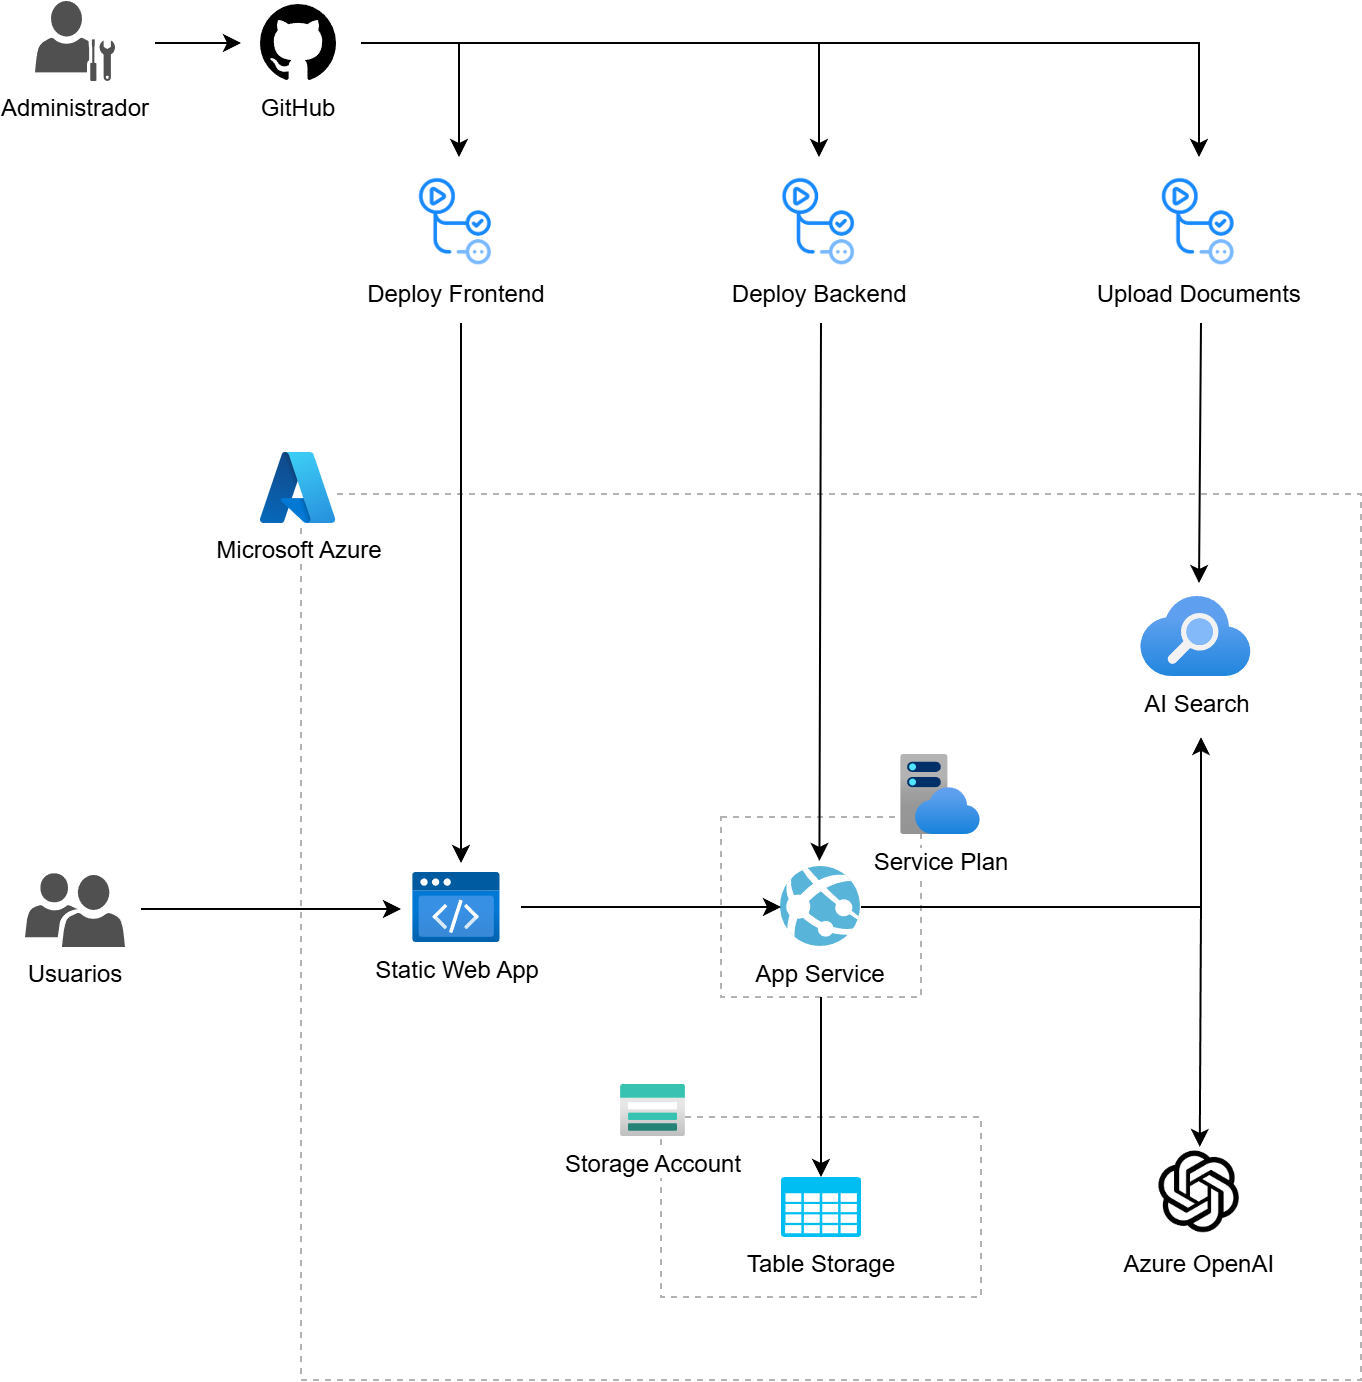
\includegraphics[scale=.55]{./Figures/arquitectura.png}
	\caption{Diagrama de arquitectura del sistema.}
	\label{fig:architecture}
\end{figure}

\vspace{8mm}

%---------------------------------------------------------------------------------------
\section{Configuración de la infraestructura en la nube}

Para garantizar el despliegue, disponibilidad y escalabilidad del sistema, se configuró una infraestructura en la nube basada en Microsoft Azure. 
A continuación, se describen los pasos principales para la configuración de cada recurso empleado en el proyecto.

\subsection{OpenAI Service}

El servicio de Azure OpenAI proporciona acceso a los potentes modelos de lenguaje de OpenAI, incluidos los más recientes. 
Estos modelos pueden adaptarse fácilmente a tareas específicas, como en este caso es la generación de contenido.

En la tabla \ref{tab:config-openai} se presenta un resumen de las configuraciones realizadas. 
Se seleccionó \textit{East US} como región, junto con el modelo de precios \textit{Standard S0}, 
adecuado para balancear el costo y el rendimiento del sistema.

Como medida de seguridad, se configuraron reglas de red para restringir el acceso únicamente al rango 
de direcciones IP del backend alojado en Azure App Service. Esto asegura que solo las solicitudes provenientes de la 
aplicación puedan acceder al modelo de lenguaje, lo que protege el servicio de accesos no autorizados.

Una vez desplegado el recurso, fue necesario seleccionar y desplegar los modelos específicos requeridos por el chatbot. 
En este caso, se optó por los siguientes modelos:

\begin{itemize}
	\item \textit{GPT-4o} como modelo de lenguaje para generación de respuestas. Este modelo está diseñado para brindar velocidad 
  y eficiencia, iguala la inteligencia de su antecesor \textit{GPT-4 Turbo}, y es notablemente más eficiente al entregar texto al 
  doble de velocidad y a la mitad del costo. Además, exhibe el rendimiento más alto en idiomas distintos del inglés en comparación 
  con los modelos de OpenAI anteriores.
	\item \textit{Ada-002} para el cálculo de \textit{embeddings} de texto. Este modelo supera a todos los modelos de \textit{embeddings} 
  anteriores en tareas de búsqueda de texto y similitud de oraciones.
\end{itemize}

Adicionalmente, es fundamental obtener el \textit{endpoint} y la \textit{key} del servicio, valores que se utilizan luego para la comunicación programática 
con Azure OpenAI. Estos datos se almacenan en el backend como variables de entorno para que el sistema pueda acceder al servicio de manera segura.

\begin{table}[h]
	\centering
	\caption[Configuración de Azure OpenAI]{Configuración de Azure OpenAI}
	\begin{tabular}{l l}    
		\toprule
		\textbf{Configuración} 	 & \textbf{Detalles} 	     \\
		\midrule
		Región                   &	East US 				 \\		
		Nivel de precios         & Standard S0				 \\
		Reglas de firewall       & Rango IP de App Service   \\
        Modelos desplegados	     & - gpt-4o				     \\
            	                 & - text-embeddings-ada-002 \\
        Credenciales	         & Endpoint y key 		     \\
		\bottomrule
		\hline
	\end{tabular}
	\label{tab:config-openai}
\end{table}

\subsection{AI Search}

Azure AI Search es un servicio de búsqueda en la nube con capacidades de inteligencia artificial integradas 
que enriquecen todo tipo de información con el fin de identificar y explorar fácilmente contenido relevante a escala.

La tabla \ref{tab:config-ai-search} presenta un resumen de las configuraciones realizadas. Se seleccionó la región de \textit{East US} y un nivel de precios 
\textit{Standard}, que ofrece hasta 50 índices para el almacenamiento y la búsqueda de documentos. En cuanto a la escala, el servicio se configuró para 
utilizar una sola unidad de búsqueda, lo cual es adecuado en principio para el volumen de consultas esperado y los requisitos de rendimiento.

Al igual que con el servicio de Azure OpenAI, se configuraron reglas de red restrictivas para mejorar la seguridad del servicio, al permitir 
únicamente el acceso desde el rango de direcciones IP asociado al backend. 

Aquí también es fundamental obtener la \textit{key} y el \textit{endpoint} del servicio para integrarlos en las variables de entorno del backend.

Es importante destacar que no es necesario crear un índice manualmente en esta etapa, ya que este será generado automáticamente como parte del pipeline de despliegue.

\begin{table}[h]
	\centering
	\caption[Configuración de Azure AI Search]{Configuración de Azure AI Search}
	\begin{tabular}{l l}    
		\toprule
		\textbf{Configuración} 	 & \textbf{Detalles} 	   \\
		\midrule
		Región                   &	East US 			   \\		
		Nivel de precios         & Standard				   \\
		Reglas de firewall       & Rango IP de App Service \\
    	Credenciales	         & Endpoint y key 		   \\
		\bottomrule
		\hline
	\end{tabular}
	\label{tab:config-ai-search}
\end{table}

\subsection{App Service}

Este servicio ofrece una plataforma completamente administrada donde es posible alojar una aplicación avanzada en la nube 
sin necesidad de manejar la infraestructura asociada. En este caso se utilizó para desplegar el backend del chatbot.

La tabla \ref{tab:config-app-service} resume la configuración principal del servicio. En primer lugar, se seleccionó un App Service Plan de categoría \textit{Basic B3}, que proporciona un poder de procesamiento de 
4 vCPU, 7 GB de memoria RAM, 10 GB de almacenamiento remoto, y permite escalar hasta 3 instancias en caso de ser necesario. 
Como entorno de ejecución, se configuró Python 3.10, mientras que como región se optó una vez más por \textit{East US}. Con el 
fin de optimizar los costos, se deshabilita la opción de redundancia zonal.

Para que la aplicación funcione correctamente, es esencial configurar un conjunto variables de entorno, que se listan en la tabla \ref{tab:config-env}. Estas 
variables incluyen las claves y los puntos de conexión de los servicios de Azure que interactúan con el backend. 

\begin{table}[h]
	\centering
	\caption[Variables de entorno en el backend]{Variables de entorno en el backend}
	\begin{tabular}{l l}    
		\toprule
		\textbf{Variable de entorno}  & \textbf{Descripción} 	                          \\
		\midrule
		openai\_api\_key              &	Clave de acceso del servicio de Azure OpenAI 	  \\		
		openai\_endpoint              & Endpoint del servicio de Azure OpenAI			  \\
		search\_key                   & Clave de acceso del servicio de Azure AI Search   \\
		search\_endpoint	          & Endpoint del servicio de Azure AI Search		  \\
        storage\_connection\_string   & Connection string de la cuenta de almacenamiento  \\
		db\_index	                  & Índice de la base de datos a utilizar		      \\
		\bottomrule
		\hline
	\end{tabular}
	\label{tab:config-env}
\end{table}

Para asegurar un monitoreo efectivo de la aplicación, se habilitó la integración con Application Insights, lo que permite un 
seguimiento detallado de las métricas de rendimiento y de uso. Adicionalmente, se configuró la opción de \textit{application logging}, 
de modo que los logs de la aplicación fueran visualizados directamente desde la terminal del App Service, facilitando la depuración 
y la supervisión continua.

\begin{table}[h]
	\centering
	\caption[Configuración de Azure App Service]{Configuración de Azure App Service}
	\begin{tabular}{l l}    
		\toprule
		\textbf{Configuración} & \textbf{Detalles} 	\\
		\midrule
		App Service Plan       & Basic B3           \\
		Runtime                & Python 3.10        \\
		Región                 & East US 			\\		
		Zone redundancy        & Deshabilitada		\\
		Application Insights   & Habilitado         \\
		Application logging	   & Filesystem			\\
		\bottomrule
		\hline
	\end{tabular}
	\label{tab:config-app-service}
\end{table}

\subsection{Static Web App}

Al utilizar este servicio, el contenido estático como HTML, CSS, JavaScript e imágenes, se distribuye globalmente desde diversos puntos 
alrededor del mundo a diferencia de un servidor web tradicional, por lo que los archivos se encuentran físicamente más cerca de los usuarios finales,
sin importar su ubicación.

La tabla \ref{tab:config-static-webapp} resume los aspectos clave de la Static Web App. Este recurso es sencillo de configurar, ya que solo requiere seleccionar un modelo de precios. En este caso, se optó por 
la versión \textit{Standard}. A diferencia de otros servicios en Azure, las Static Web Apps se despliegan globalmente, por lo que no es necesario especificar una región. 
Además, ya que todas las conexiones con otros servicios son manejadas exclusivamente por el backend, la única variable de entorno requerida 
es la URL de la API, lo que simplifica la configuración.

Es importante obtener el \textit{deployment token} asociado al recurso, que será necesario más adelante para configurar el pipeline de despliegue automático, 
permitiendo la autenticación y el despliegue seguro desde GitHub.

\begin{table}[h]
	\centering
	\caption[Configuración de Azure App Service]{Configuración de Azure App Service}
	\begin{tabular}{l l}    
		\toprule
		\textbf{Configuración} 	& \textbf{Detalles} \\
		\midrule
		Nivel de precios        & Standard          \\
		Región                  & Global 			\\		
		Variables de entorno    & URL del backend	\\
		Credenciales            & Deployment token  \\
		\bottomrule
		\hline
	\end{tabular}
	\label{tab:config-static-webapp}
\end{table}

\subsection{Table Storage}

Azure Table Storage es un servicio que almacena datos estructurados no relacionales (también conocidos como datos NoSQL) en la nube, que almacena claves/atributos 
con un diseño sin esquemas. En el contexto de este trabajo se utilizó para almacenar el feedback de los usuarios acerca de las respuestas provistas por el chatbot.

La tabla \ref{tab:config-table-storage} resume la configuración principal de este recurso. Primeramente, fue necesario desplegar una Storage Account en la región \textit{East US}, para así mantener la consistencia con los demás 
recursos del sistema. Se seleccionó una performance de tipo \textit{Standard}, adecuada para las necesidades de la aplicación.

En cuanto a la redundancia de los datos, se eligió la oferta de redundancia local, una alternativa rentable que asegura que los datos 
estén replicados dentro de un único centro de datos en la misma región, reduciendo costos sin comprometer la disponibilidad básica.

Una vez que la cuenta de almacenamiento fue desplegada, se procedió a crear la tabla que almacenará los resultados 
recopilados a través del sistema. Es importante obtener la \textit{connection string} asociada al recurso, ya que será 
necesaria para conectar la aplicación con la tabla y permitir el acceso programático. 

\begin{table}[h]
	\centering
	\caption[Configuración de Azure Table Storage]{Configuración de Azure Table Storage}
	\begin{tabular}{l l}    
		\toprule
		\textbf{Configuración} 	 & \textbf{Detalles} 	      \\
		\midrule
		Región                   &	East US 				  \\		
		Performance	             &  Standard				  \\
		Redundancia	             &  Locally-redundant storage \\
		Credenciales             &  Connection string         \\
		Nombre de la tabla       &	FeedbackTable             \\
		\bottomrule
		\hline
	\end{tabular}
	\label{tab:config-table-storage}
\end{table}

%---------------------------------------------------------------------------------------
\section{Procesamiento de los documentos}

La finalidad del procesamiento de documentos es transformar archivos de texto y PDF en un formato que facilite su búsqueda y análisis mediante 
herramientas de inteligencia artificial. Este flujo de trabajo incluye el uso de modelos de \textit{embeddings} para convertir el texto en 
representaciones vectoriales, y su posterior inserción en una base de datos vectorial. Para ello, se desarrolló un script en Python que asegura 
un manejo eficiente de grandes volúmenes de datos, al implementar mecanismos para distribuir las solicitudes a la API de Azure Search y evitar 
superar sus límites de tasa de uso, además de optimizar el almacenamiento en el índice de búsqueda.

\subsection{Importación de bibliotecas y configuración inicial}

El script comienza con la importación de las bibliotecas necesarias para realizar el procesamiento de documentos. Se utilizan paquetes específicos 
que integran funciones avanzadas para trabajar con \textit{embeddings}, carga de documentos, y búsqueda por similitud. El módulo \textit{nltk} es esencial 
para el procesamiento de texto en lenguaje natural, al proporcionar herramientas de tokenización y etiquetado de texto.

\begin{lstlisting}[label=cod:update-db-1,caption=Importación de bibliotecas y configuración inicial.]
	import os
	import requests
	from langchain_openai import AzureOpenAIEmbeddings
	from langchain_google_genai import GoogleGenerativeAIEmbeddings
	from langchain_community.vectorstores.azuresearch import AzureSearch
	from langchain_text_splitters import RecursiveCharacterTextSplitter
	from langchain_community.document_loaders import UnstructuredMarkdownLoader, PyPDFLoader
	import nltk
	import time

	nltk.download('punkt_tab')
	nltk.download('averaged_perceptron_tagger_eng')
\end{lstlisting}

\subsection{Configuración del índice de búsqueda}

Antes de insertar documentos en la base de datos, es necesario realizar una limpieza para eliminar cualquier dato previo. La función 
\textit{delete\_index} se encarga de esta tarea, enviando una solicitud de tipo \textit{DELETE} a la API de Azure Search para borrar todos 
los documentos de un índice específico.

\begin{lstlisting}[label=cod:update-db-2,caption=Configuración del índice de búsqueda.]
	def delete_index(azure_search_endpoint, azure_search_key, index_name):
		url = f"{azure_search_endpoint}/indexes('{index_name}')?api-version=2023-11-01"
		headers = {
			"Content-Type": "application/json",
			"api-key": f"{azure_search_key}"
		}
		response = requests.delete(url, headers=headers)
		if response.status_code == 204:
			print("All documents deleted successfully.")
		else:
			print(f"Failed to delete documents. Status code: {response.status_code}, Response: {response.text}")
\end{lstlisting}

Este paso es esencial para asegurar que los datos insertados sean consistentes con los documentos procesados más recientemente, evitando 
duplicación de información y permitiendo un índice limpio.

\subsection{Configuración del modelo de \textit{embeddings}}

La selección del modelo de \textit{embeddings} depende de una variable de entorno. El script soporta tanto modelos de Azure OpenAI como de Google. 
Según el modelo especificado, se inicializa una instancia de \textit{AzureOpenAIEmbeddings} o \textit{GoogleGenerativeAIEmbeddings}.

\begin{lstlisting}[label=cod:update-db-3,caption=Configuración del modelo de \textit{embeddings}.]
	if os.getenv("EMBEDDINGS_MODEL") == "openai":
		embeddings = AzureOpenAIEmbeddings(model="ada-002", openai_api_version="2024-06-01")
	elif os.getenv("EMBEDDINGS_MODEL") == "google":    
		embeddings = GoogleGenerativeAIEmbeddings(model="models/embedding-001")
	else:
		embeddings = AzureOpenAIEmbeddings(model="ada-002", openai_api_version="2024-06-01")
\end{lstlisting}

\subsection{Conexión con la base de datos}

Una vez configurado el modelo de \textit{embeddings}, el siguiente paso es instanciar una conexión con el índice de Azure Search. 
Esto permite la interacción directa con el índice y la inserción de documentos procesados.

\begin{lstlisting}[label=cod:update-db-4,caption=Conexión con la base de datos.]
	azure_search = AzureSearch(
		azure_search_endpoint=os.getenv("AZURE_SEARCH_URI"),
		azure_search_key=os.getenv("AZURE_SEARCH_KEY"),
		index_name=index_name,
		embedding_function=embeddings.embed_query
	)
\end{lstlisting}

Este objeto se utiliza posteriormente en el flujo para agregar documentos en el índice de búsqueda, una vez que hayan sido procesados y transformados en \textit{embeddings}.

\subsection{Divisor de texto}

Para manejar eficientemente documentos extensos, el script utiliza un divisor de texto para separar el contenido en fragmentos manejables 
de hasta 512 caracteres con un solapamiento de 64 caracteres entre fragmentos consecutivos. Este solapamiento asegura la continuidad del
contexto en los fragmentos resultantes.

El script busca archivos en la carpeta \textit{knowledge-base} y aplica distintos \textit{loaders} según el tipo de archivo (PDF o Markdown). Luego, 
cada archivo se divide en fragmentos utilizando el divisor de texto configurado previamente.

\begin{lstlisting}[label=cod:update-db-5,caption=Divisor de texto.]
	splitter = RecursiveCharacterTextSplitter(chunk_size=512, chunk_overlap=64)

	for root, dirs, files in os.walk('knowledge-base'):
    for file in files:
        file_path = os.path.join(root, file)
        if file.endswith('.pdf'):
            data_loader = PyPDFLoader(file_path)
        elif file.endswith('.md'):
            data_loader = UnstructuredMarkdownLoader(file_path)
        file_chunks = data_loader.load_and_split(text_splitter=splitter)
        print(f"{file_path} splitted into {len(file_chunks)} chunks")
\end{lstlisting}

\subsection{Inserción en lotes}

Para evitar alcanzar el límite de uso de la API, los fragmentos se insertan en el índice en lotes pequeños, con una demora entre cada lote. 
La función \textit{batch\_insert\_chunks} controla esta inserción en lotes, estableciendo un tamaño de lote y un tiempo de espera entre lotes.

\begin{lstlisting}[label=cod:update-db-6,caption=Inserción en lotes.]
	def batch_insert_chunks(chunks,batch_size=5,delay_between_batches=3):
    batch_count=0
    inserted_ids = []
    for i in range(0, len(chunks), batch_size):
        batch = chunks[i:i+batch_size]
        batch_count += 1
        inserted_ids_batch = azure_search.add_documents(batch)
        inserted_ids.extend(inserted_ids_batch)
        print(f"Inserted batch #{batch_count} ({len(inserted_ids_batch)} documents)")
        time.sleep(delay_between_batches)
    return inserted_ids
\end{lstlisting}

La inserción en lotes es un aspecto clave del diseño, ya que permite manejar eficientemente grandes volúmenes de datos sin interrumpir
el flujo debido a límites de solicitud.

\vspace{8mm}

%---------------------------------------------------------------------------------------
\section{Lógica de generación aumentada por recuperación}

El sistema RAG se compone de dos etapas principales:

\begin{itemize}
	\item Fase de recuperación: Se realiza una búsqueda semántica en la base de datos vectorial para identificar 
	los fragmentos más relevantes a partir de una consulta.
	\item Fase de generación: Los fragmentos recuperados se combinan con la consulta del usuario y se utilizan 
	como contexto para un modelo de lenguaje grande (LLM), que genera una respuesta contextualizada.
\end{itemize}

Este enfoque aprovecha lo mejor de ambos mundos: la precisión en la recuperación de datos específicos y 
la capacidad generativa avanzada de los LLM.

\subsection{Fase de recuperación}

La recuperación de información es una pieza clave del sistema RAG, encargada de encontrar los fragmentos más relevantes de la base de datos vectorial.

Para ello se desarrolló la clase \textit{Retriever}, cuyo código se muestra a continuación. 

\begin{lstlisting}[label=cod:retriever,caption=Clase \textit{Retriever}.]
	class Retriever():
	
		def __init__(self):
			# Embeddings model instantiation
			if os.getenv("EMBEDDINGS_MODEL") == "openai":
				self.embeddings = AzureOpenAIEmbeddings(model="ada-002", openai_api_version="2024-06-01")
			elif os.getenv("EMBEDDINGS_MODEL") == "google":    
				self.embeddings = GoogleGenerativeAIEmbeddings(model="models/embedding-001")
			else:
				self.embeddings = AzureOpenAIEmbeddings(model="ada-002", openai_api_version="2024-06-01")
	
			# Vector store instantiation
			self.vstore = AzureSearch(
				azure_search_endpoint=os.getenv("AZURE_SEARCH_URI"),
				azure_search_key=os.getenv("AZURE_SEARCH_KEY"),
				index_name=os.getenv("DB_INDEX"),
				embedding_function=self.embeddings.embed_query
			)
	
		def invoke(self, query):
			# Run a similarity search on the database for the given query
			docs = self.vstore.similarity_search(query['input'], k=3)
			print(docs)
			return self.format_docs(docs)
		
		def format_docs(self, docs):
			# Put together the results of the similarity search into one chunk of text
			return "\n\n".join(doc.page_content for doc in docs)
\end{lstlisting}

En el constructor se inicializa el modelo de \textit{embeddings} y se establece la conexión con la base de datos vectorial en Azure Search.

El método \textit{invoke} realiza una búsqueda semántica en la base de datos y devuelve los documentos más relevantes. El método utiliza la 
función \textit{similarity\_search} para recuperar los tres fragmentos más relevantes (k=3). Posteriormente, los fragmentos se 
formatean a través del método \textit{format\_docs} en un texto único que servirá como contexto para la fase de generación. Esta 
estructura garantiza que el modelo de generación reciba un contexto consolidado y relevante.

\subsection{Fase de generación}

La fase de generación utiliza los fragmentos recuperados para producir respuestas contextuales a las consultas del usuario.

Para ello se desarrolló la clase \textit{Generator}, cuyo código se muestra a continuación.

\begin{lstlisting}[label=cod:generator,caption=Clase \textit{Generator}.]
	class Generator():

		def __init__(self, retriever):
			# Instantiate a pre-trained Large Language Model from Azure OpenAI
			self.llm = AzureChatOpenAI(
				deployment_name="gpt-4o",
				api_version="2023-06-01-preview"
			)

			# The system prompt guides the model on how to respond
			self.system_prompt = (
				"You are an AI assistant for question-answering tasks."
				"You are able to answer questions related to Fabian's final project for his master degree in AI."
				"If someone asks, 'What can I ask you about?' or other similar questions, respond with the above topics."
				"If you're unsure, use the following pieces of retrieved context to answer the question." 
				"If you don't know the answer, say that you don't know."
				"If a question does not relate to Fabian's project, respond with: 'This question falls outside of my knowledge base'." 
				"Use three sentences maximum and keep the answer concise."
				"\n\n"
				"{context}"
			)

			# The prompt puts together the system prompt with the user question
			self.prompt = ChatPromptTemplate.from_messages(
				[
					("system", self.system_prompt),
					("human", "{question}"),
				]
			)

			# The parser just plucks the string content out of the LLM's output message
			self.parser = StrOutputParser()

			# The chain orchestrates the whole flow
			self.rag_chain = (
				{"context": retriever.invoke, "question": RunnablePassthrough()}
				| self.prompt
				| self.llm
				| self.parser
			)


		def invoke(self, user_question):
			# Run the chain and returns the answer generated by the LLM
			answer = self.rag_chain.invoke({"input": user_question})
			return answer
\end{lstlisting}

En el constructor se inicializan todos los componentes fundamentales: un modelo de lenguaje grande en Azure OpenAI,
el \textit{prompt} del sistema, y una cadena (\textit{rag\_chain}) que organiza el flujo completo de la consulta, 
desde la recuperación de fragmentos hasta la generación de la respuesta. Esta estructura 
garantiza que los datos recuperados se integren con la consulta del usuario antes de pasar al modelo generativo.

El \textit{prompt} establece las instrucciones que guían al modelo en la generación de respuestas, al definir 
tanto el tono como las reglas que debe seguir. Este está diseñado para:

\begin{enumerate}
	\item Concientizar al chatbot sobre su dominio de conocimiento.
    \item Incluir solo información del contexto recuperado.
    \item Evitar responder a consultas fuera del dominio del chatbot.
    \item Limitar las respuestas a tres oraciones.
\end{enumerate}

El método \textit{invoke} utiliza la cadena para procesar la consulta del usuario y generar la respuesta final.

%---------------------------------------------------------------------------------------
\section{Implementación de la API}

La API desarrollada con FastAPI es el puente entre la interfaz de usuario y las funcionalidades del sistema. La 
tabla \ref{tab:api} detalla los endpoints implementados.

\begin{table}[h]
	\centering
	\caption[Diseño de la API]{Diseño de la API}
	\begin{tabular}{l c c}    
		\toprule
		\textbf{Endpoint} 	     & \textbf{Método} 	& \textbf{Ruta}  \\
		\midrule
		Generación de respuesta  &  POST 		    & /api/ask       \\		
		Registro de feedback     &  POST		    & /api/feedback  \\
		Consulta de feedback	 &  GET             & /api/feedback  \\
		Prueba                   &  GET             & /api/ping      \\
		\bottomrule
		\hline
	\end{tabular}
	\label{tab:api}
\end{table}

\subsection{Endpoint de generación de respuestas}

Este endpoint recibe la consulta del usuario e invoca el proceso RAG para generar una respuesta en lenguaje natural.

\begin{lstlisting}[label=cod:api-1,caption=Endpoint de generación de respuestas.]
	@app.post("/api/ask")
	def generate_answer(body: Prompt):
		try:
			answer = generator.invoke(body.prompt)
			return {"question": body.prompt, "answer": answer}
		except Exception as e:
			raise HTTPException(status_code=500, detail=f"Error: {e}")	
\end{lstlisting}

\subsection{Endpoint de registro de feedback}

Este endpoint permite a los usuarios enviar su opinión sobre una interacción, es decir, si están o no satisfechos con 
la respuesta entregada por el chatbot. Los datos se almacenan en Azure Table Storage.
El propósito es capturar la percepción del usuario sobre las respuestas generadas, permitiendo evaluar y mejorar el sistema.

\begin{lstlisting}[label=cod:api-2,caption=Endpoint de registro de feedback.]
	@app.post("/api/feedback")
	async def store_feedback(feedback: Feedback):
		entity = TableEntity()
		entity["PartitionKey"] = "likes" if feedback.like else "hates"
		entity["RowKey"] = str(uuid.uuid4())
		entity["Question"] = feedback.question
		entity["Answer"] = feedback.answer
	
		try:
			table_client.create_entity(entity=entity)
			return {"message": "Feedback stored successfully."}
		except Exception as e:
			raise HTTPException(status_code=500, detail=f"Error: {e}")
	
\end{lstlisting}

\subsection{Endpoint de consulta de feedback}

Este endpoint retorna estadísticas sobre el feedback registrado por los usuarios, al indicar la cantidad de interacciones 
positivas y negativas. El propósito es ofrecer estadísticas que permitan monitorear el rendimiento del sistema y 
la satisfacción del usuario.

\begin{lstlisting}[label=cod:api-3,caption=Endpoint de consulta de feedback.]
	@app.get("/api/feedback")
	async def get_feedback_count():
		try:
			likes_count = len(list(table_client.query_entities(query_filter="PartitionKey eq 'likes'")))
			hates_count = len(list(table_client.query_entities(query_filter="PartitionKey eq 'hates'")))
	
			return {"likes": likes_count, "hates": hates_count}
		except Exception as e:
			raise HTTPException(status_code=500, detail=f"Error: {e}")	
\end{lstlisting}

\subsection{Endpoint de prueba}

Este endpoint verifica que la API esté operativa devolviendo una respuesta sencilla. Su propósito es 
validar la conectividad con la API y confirmar que el sistema está funcionando correctamente.

\begin{lstlisting}[label=cod:api-4,caption=Endpoint de prueba.]
	@app.get("/api/ping")
	def ping():
		return "pong"
\end{lstlisting}

%---------------------------------------------------------------------------------------
\section{Implementación de la interfaz de usuario}

%---------------------------------------------------------------------------------------
\section{Pipelines de despliegue automático}
% Chapter Template

\chapter{Ensayos y resultados} % Main chapter title

\label{Chapter4} % Change X to a consecutive number; for referencing this chapter elsewhere, use \ref{ChapterX}

%----------------------------------------------------------------------------------------

Todos los capítulos deben comenzar con un breve párrafo introductorio que indique cuál es el contenido que se encontrará al leerlo.  La redacción sobre el contenido de la memoria debe hacerse en presente y todo lo referido al proyecto en pasado, siempre de modo impersonal.

%---------------------------------------------------------------------------------------
\section{Ensayo de modelos}
 
%---------------------------------------------------------------------------------------
\section{Ensayo de embeddings}

%---------------------------------------------------------------------------------------
\section{Ensayo de bases de datos}

%---------------------------------------------------------------------------------------
\section{Casos de uso}

%---------------------------------------------------------------------------------------
\section{Validación de requerimientos}

 
% Chapter Template

\chapter{Conclusiones} % Main chapter title

\label{Chapter5} % Change X to a consecutive number; for referencing this chapter elsewhere, use \ref{ChapterX}

%----------------------------------------------------------------------------------------

Todos los capítulos deben comenzar con un breve párrafo introductorio que indique cuál es el contenido que se encontrará al leerlo.  La redacción sobre el contenido de la memoria debe hacerse en presente y todo lo referido al proyecto en pasado, siempre de modo impersonal.

%---------------------------------------------------------------------------------------
\section{Resultados}


%----------------------------------------------------------------------------------------
\section{Trabajo futuro}
 

%----------------------------------------------------------------------------------------
%	CONTENIDO DE LA MEMORIA  - APÉNDICES
%----------------------------------------------------------------------------------------

\appendix % indicativo para indicarle a LaTeX los siguientes "capítulos" son apéndices

% Incluir los apéndices de la memoria como archivos separadas desde la carpeta Appendices
% Descomentar las líneas a medida que se escriben los apéndices

%\include{Appendices/AppendixA}
%\include{Appendices/AppendixB}
%\include{Appendices/AppendixC}

%----------------------------------------------------------------------------------------
%	BIBLIOGRAPHY
%----------------------------------------------------------------------------------------

\Urlmuskip=0mu plus 1mu\relax
\raggedright
\printbibliography[heading=bibintoc]

%----------------------------------------------------------------------------------------

\end{document}  
